\documentclass[conference]{IEEEtran}
\IEEEoverridecommandlockouts
% The preceding line is only needed to identify funding in the first footnote. If that is unneeded, please comment it out.
\usepackage{cite}
\usepackage{amsmath,amssymb,amsfonts}
\usepackage{algorithmic}
\usepackage{graphicx}
\usepackage{textcomp}
\usepackage{float}
\usepackage{multirow, array}
\renewcommand{\arraystretch}{1.25} % Incremento del espacio entre filas
%\usepackage{soul} % Para resaltar
%\usepackage{float}

%\usepackage{xcolor}
%\sethlcolor{yellow} % Cambiar color del resaltado a amarillo
% packages to highlight
\usepackage{siunitx}
\usepackage{soul}
\usepackage{color}
\newcommand{\hlcyan}[1]{{\sethlcolor{cyan}\hl{#1}}}
\newcommand{\hlgreen}[1]{{\sethlcolor{green}\hl{#1}}}
\newcommand{\hlred}[1]{{\sethlcolor{red}\hl{#1}}}
\newcommand{\hlblue}[1]{{\sethlcolor{blue}\hl{#1}}}
\newcommand{\hlmag}[1]{{\sethlcolor{magenta}\hl{#1}}}

\def\BibTeX{{\rm B\kern-.05em{\sc i\kern-.025em b}\kern-.08em
    T\kern-.1667em\lower.7ex\hbox{E}\kern-.125emX}}
\begin{document}



\title{Generación de Señales para el Subsistema de Digitalización en el Banco de Pruebas de la Tarjeta DAPHNE en el Experimento DUNE\\
{\footnotesize \textsuperscript \n LATS2025 - 26th IEEE Latin - American Test Symposium}
%\thanks{Identify applicable funding agency here. If none, delete this.}
}

\author{\IEEEauthorblockN{1\textsuperscript{st} Juan Fajardo}
\IEEEauthorblockA{GICM - \textit{Master's in Engineering student} \\
\textit{Engineering Faculty}\\
\textit{Universidad de Antioquia}\\
Medellín, Colombia \\
https://orcid.org/0009-0007-7711-7759}
\and

\IEEEauthorblockN{2\textsuperscript{nd} Jerónimo López\orcidC{}}
\IEEEauthorblockA{GICM - \textit{Undergraduate Physics Student} \\
\textit{Exact and Natural Sciences Faculty}\\
\textit{Universidad de Antioquia}\\
Medellín, Colombia \\
https://orcid.org/0009-0003-1900-3172}
\and

\IEEEauthorblockN{3\textsuperscript{rd} Valentina Ródriguez}
\IEEEauthorblockA{GICM - \textit{Undergraduate Physics Student} \\
\textit{Exact and Natural Sciences Faculty}\\
\textit{Universidad de Antioquia}\\
Medellín, Colombia \\
https://orcid.org/0009-0009-5214-1976}
\and

\IEEEauthorblockN{4\textsuperscript{th} Valentina Restrepo}
\IEEEauthorblockA{GICM - \textit{Undergraduate Engineering Student} \\
\textit{Engineering Faculty}\\
\textit{Universidad de Antioquia}\\
Medellín, Colombia \\
https://orcid.org/0000-0003-1747-0095}
\and

\IEEEauthorblockN{5\textsuperscript{th} Fabian Andres Castaño}
\IEEEauthorblockA{GICM - \textit{Physics Institute} \\
\textit{Exact and Natural Sciences Faculty}\\
\textit{Universidad de Antioquia}\\
Medellín, Colombia \\
fabian.castano@udea.edu.co\\
https://orcid.org/0000-0001-8014-4773}
}


\maketitle

\begin{abstract}
El experimento DUNE (Deep Underground Neutrino Experiment) estudia neutrinos, partículas fundamentales que interactúan débilmente con la materia. Este artículo presenta el desarrollo de un banco de pruebas automatizado para evaluar las tarjetas DAPHNE, esenciales en la adquisición de datos del experimento. La metodología incluye la generación de señales digitales mediante diseños en HDL implementados en FPGA, disparados por pulsos del ESP32, y convertidos a señales analógicas en su DAC, evaluadas con el Analog Discovery 2. Los resultados evidencian la correcta implementación de diseños HDL basados en datos predefinidos y ecuaciones en diferencias. La comparación muestra que el modelo con ecuaciones en diferencias tiene mayor capacidad de procesamiento dinámico a costa de más recursos, mientras que el diseño con datos predefinidos es más eficiente. Este desarrollo optimiza la evaluación de DAPHNE, mejorando su confiabilidad y adaptabilidad a las condiciones extremas del experimento DUNE.
\end{abstract}

\begin{IEEEkeywords}
FPGA (Field-Programmable Gate Array), Data acquisition, Signal generation, Analog-to-digital conversion, Embedded systems
\end{IEEEkeywords}






%%%%%%%%%%%%%%%%%%%%%%%%%%%%%%%%%%%%%%%%%%%%%%%%%%%%%%%%
%% Introduccion
%%%%%%%%%%%%%%%%%%%%%%%%%%%%%%%%%%%%%%%%%%%%%%%%%%%%%%%%

\section{Introduction}

% Texto original
%
\hl{comentario}
\hlgreen{Aceptado}
E\hlcyan{Idea}
\hlred{Error}
\hlmag{Idea}
\hlblue{otros}

El experimento DUNE (\textit{Deep Underground Neutrino Experiment}) tiene como propósito principal la observación y el estudio detallado de los neutrinos, partículas fundamentales cuya interacción extremadamente débil con la materia, representada por su baja sección eficaz de interacción ($10^{-45} \, \si{\meter^2}$), los hace sumamente difíciles de detectar \cite{Mishra1990}. Sin embargo, estas partículas tienen el potencial de revelar respuestas fundamentales sobre los orígenes y la evolución del universo. En este contexto, el consorcio encargado del Sistema de Detección de Fotones (\textit{PDS}) ha diseñado y desarrollado una plataforma tecnológica de alto rendimiento conocida como \textit{DAPHNE} (\textit{Detector electronics for Acquiring Photons from Neutrinos}). Este sistema desempeña un papel crucial en la adquisición y procesamiento de datos dentro del \textit{Far Detector}, asegurando una recopilación precisa y eficiente de la información científica necesaria, incluso bajo condiciones operativas extremas \cite{Abi2020}.


Como uno de los principales proyectos estratégicos en el ámbito de la física de partículas, DUNE se encuentra respaldado por el Panel de Priorización de Proyectos de Física de Partículas (\textit{P5}), que en su informe de 2023 destacó la importancia de las fases I y II para avanzar en la comprensión de los neutrinos y sus mecanismos de interacción y producción \cite{DUNE_Phase_II}, \cite{P5_Report}. El \textit{Far Detector} de DUNE consiste en seis criostatos que contienen un total de 70 kilotoneladas de argón líquido (\textit{LAr}), situados a 1.5 km bajo la superficie en Sanford, Dakota del Sur. Este entorno plantea retos significativos para el mantenimiento y la reparación, dadas las condiciones ambientales extremas y el acceso limitado a las instalaciones \cite{Abi2020}. 

El sistema \textit{DAPHNE} está compuesto por 150 tarjetas electrónicas, cada una de las cuales integra cinco AFE5808A (\textit{Analog Front End}), diseñados para amplificar, filtrar y digitalizar señales provenientes de los SiPM en las X-Arapucas. Cada tarjeta cuenta con 40 canales de adquisición que operan a una velocidad de muestreo de 62.5 Msps con una resolución de 14 bits, generando un volumen de datos agregado estimado en 450 Gbps. Esto demuestra la capacidad de \textit{DAPHNE} para gestionar la complejidad y los altos requisitos de datos asociados al experimento \hlblue{otros\cite{SystemSpecs2023}}.

Desde su primera implementación en 2019, el sistema \textit{DAPHNE} ha evolucionado a través de tres versiones, cada una desarrollada para satisfacer las crecientes demandas del \textit{PDS}. La arquitectura inicial integró un microcontrolador STM32H753II para el \textit{Slow Control} y una FPGA Artix-7 responsable del \textit{Fast Data Acquisition}. El microcontrolador supervisa parámetros clave, como tensiones, ajustes de ganancia y configuraciones de periféricos, utilizando interfaces estándar como USART, SPI e I2C. Mientras tanto, la FPGA Artix-7 maneja el procesamiento y la transmisión de datos de alta velocidad \cite{STM32H753II}. 

En 2022, la versión 2 de \textit{DAPHNE} introdujo enlaces de alta velocidad basados en Gigabit Ethernet, gestionados mediante el protocolo TCP/IP. En 2023, la versión 3 presentó una arquitectura optimizada y compacta, utilizando un \textit{System on Module} Kria K26, que incorpora un coprocesador ARM y una FPGA embebida, mejorando significativamente la eficiencia del sistema \cite{DUNE_Far_Detector}. 

El ambiente de operación en Sanford representa desafíos técnicos considerables, como temperaturas extremas, alta humedad, exposición a radiación y acceso limitado a las cavernas subterráneas. Adicionalmente, los protocolos de prueba actuales de \textit{DAPHNE} no están completamente estandarizados, lo que genera una dependencia de operadores especializados y puede derivar en errores sistemáticos. Estas dificultades prolongan los tiempos de validación y aumentan los costos, poniendo en riesgo el cronograma del experimento \cite{Esteban_Ferrer}.

Para superar estas limitaciones, el Grupo de Instrumentación Científica y Microelectrónica (\textit{GICM}) de la Universidad de Antioquia está desarrollando un banco de pruebas automatizado, diseñado bajo protocolos de medición estandarizados. Este sistema tiene como objetivo optimizar los tiempos de prueba, minimizar las inconsistencias y mitigar riesgos de implementación. Además, se plantea la integración de herramientas de inteligencia artificial para analizar patrones en las condiciones operativas de las tarjetas \textit{DAPHNE}, lo que permitirá implementar estrategias de mantenimiento preventivo, reducir la incidencia de fallas y minimizar la intervención humana \hlblue{otros} \cite{GICMDevelopment2023}.

El banco de pruebas permitirá realizar mediciones de parámetros críticos, como los voltajes de operación, las impedancias de las tarjetas y el desempeño de los sistemas de digitalización y transmisión de señales. Este artículo se centra en los avances logrados en la evaluación de los sistemas de digitalización, enfocándose en la medición de la frecuencia de operación de los subsistemas de \textit{DAPHNE}, evaluando su estabilidad y confiabilidad mediante el uso de matrices de puertas lógicas programables (\textit{FPGA}), herramientas clave para asegurar el éxito del experimento DUNE.

% texto en ingles
%%%%%%%%%%%%%%%%%%%%%%%%%%%%%%%%%%%%%%%%%%%
%% Texto en ingles
%%%%%%%%%%%%%%%%%%%%%%%%%%%%%%%%%%%%%%%%%%%



%%%%%%%%%%%%%%%%%%%%%%%%%%%%%%%%%%%%%%%%%%%%%%%%%%%%%%%%%%%%
%%%%%%%%%%%%%%%%%%%%%%%%%%%%%%%%%%%%%%%%%%%%%%%%%%%%%%%%%%%%
%% Introduccion al experimento
%%%%%%%%%%%%%%%%%%%%%%%%%%%%%%%%%%%%%%%%%%%%%%%%%%%%%%%%%%%%
%%%%%%%%%%%%%%%%%%%%%%%%%%%%%%%%%%%%%%%%%%%%%%%%%%%%%%%%%%%%

The DUNE experiment (\textit{Deep Underground Neutrino Experiment}) aims primarily at the observation and detailed study of neutrinos, fundamental particles whose extremely weak interaction with matter, represented by their low cross-section of interaction ($10^{-45}$\SI{}{\meter^2}), makes them extremely difficult to detect \cite{Mishra1990}. However, these particles have the potential to reveal fundamental insights into the origins and evolution of the universe. In this context, the consortium responsible for the Photon Detection System (\textit{PDS}) has designed and developed a high-performance technological platform known as \textit{DAPHNE} (\textit{Detector electronics for Acquiring Photons from Neutrinos}). This system plays a crucial role in the acquisition and processing of data within the \textit{Far Detector}, ensuring accurate and efficient collection of the necessary scientific information, even under extreme operational conditions \cite{Abi2020}. % El experimento DUNE (\textit{Deep Underground Neutrino Experiment}) tiene como propósito principal la observación y el estudio detallado de los neutrinos, partículas fundamentales cuya interacción extremadamente débil con la materia, representada por su baja sección eficaz de interacción ($10^{-45}$\SI{}{\meter^2}), los hace sumamente difíciles de detectar \cite{Mishra1990}. Sin embargo, estas partículas tienen el potencial de revelar respuestas fundamentales sobre los orígenes y la evolución del universo. En este contexto, el consorcio encargado del Sistema de Detección de Fotones (\textit{PDS}) ha diseñado y desarrollado una plataforma tecnológica de alto rendimiento conocida como \textit{DAPHNE} (\textit{Detector electronics for Acquiring Photons from Neutrinos}). Este sistema desempeña un papel crucial en la adquisición y procesamiento de datos dentro del \textit{Far Detector}, asegurando una recopilación precisa y eficiente de la información científica necesaria, incluso bajo condiciones operativas extremas \cite{Abi2020}.



As one of the main strategic projects in the field of particle physics, \textit{DUNE} is supported by the Particle Physics Project Prioritization Panel (\textit{P5}), which in its 2023 report emphasized the importance of Phases I and II to advance the understanding of neutrinos and their mechanisms of interaction and production \cite{DUNE_Phase_II}, \cite{P5_Report}. The \textit{Far Detector} of \textit{DUNE} consists of six cryostats containing a total of $70$ kilotons of liquid argon (\textit{LAr}), located \SI{1.5}{\kilo\meter} underground at Sanford, South Dakota. This environment presents significant challenges for maintenance and repair due to the extreme environmental conditions and limited access to the facilities \cite{Abi2020}. % Como uno de los principales proyectos estratégicos en el ámbito de la física de partículas, DUNE se encuentra respaldado por el Panel de Priorización de Proyectos de Física de Partículas (\textit{P5}), que en su informe de 2023 destacó la importancia de las fases I y II para avanzar en la comprensión de los neutrinos y sus mecanismos de interacción y producción \cite{DUNE_Phase_II}, \cite{P5_Report}. El \textit{Far Detector} de DUNE consiste en seis criostatos que contienen un total de 70 kilotoneladas de argón líquido (\textit{LAr}), situados a 1.5 km bajo la superficie en Sanford, Dakota del Sur. Este entorno plantea retos significativos para el mantenimiento y la reparación, dadas las condiciones ambientales extremas y el acceso limitado a las instalaciones \cite{Abi2020}. 


%%%%%%%%%%%%%%%%%%%%%%%%%%%%%%%%%%%%%%%%%%%%%%%%%%%%%%%%%%%%
%%%%%%%%%%%%%%%%%%%%%%%%%%%%%%%%%%%%%%%%%%%%%%%%%%%%%%%%%%%%
%% Contexto del problema de DAPHNE
%%%%%%%%%%%%%%%%%%%%%%%%%%%%%%%%%%%%%%%%%%%%%%%%%%%%%%%%%%%%
%%%%%%%%%%%%%%%%%%%%%%%%%%%%%%%%%%%%%%%%%%%%%%%%%%%%%%%%%%%%


The \textit{DAPHNE} system consists of $150$ electronic boards, each of which integrates five AFE5808A (\textit{Analog Front End}) chips, designed to amplify, filter, and digitize signals from the SiPMs in the X-Arapucas \cite{Abi2020, Falcone2021}. Each board has $40$ acquisition channels that operate at a sampling rate of $62.5$ Msps with a $14$-bit resolution, generating an estimated aggregated data volume of $450$ Gbps. This demonstrates the ability of \textit{DAPHNE} to manage the complexity and high data requirements associated with the experiment \cite{Abi_2020, Abi2020C, Abi2020}. % El sistema \textit{DAPHNE} está compuesto por 150 tarjetas electrónicas, cada una de las cuales integra cinco AFE5808A (\textit{Analog Front End}), diseñados para amplificar, filtrar y digitalizar señales provenientes de los SiPM en las X-Arapucas. Cada tarjeta cuenta con 40 canales de adquisición que operan a una velocidad de muestreo de 62.5 Msps con una resolución de 14 bits, generando un volumen de datos agregado estimado en 450 Gbps. Esto demuestra la capacidad de \textit{DAPHNE} para gestionar la complejidad y los altos requisitos de datos asociados al experimento \hlcyan{otros} \cite{SystemSpecs2023}.


%%%%%%%%%%%%%%%%%%%%%%%%%%%%%%%%%%%%%%%%%%%%%%%%%%%%%%%%%%%%
%%%%%%%%%%%%%%%%%%%%%%%%%%%%%%%%%%%%%%%%%%%%%%%%%%%%%%%%%%%%
%% Versiones de DAPHNE
%%%%%%%%%%%%%%%%%%%%%%%%%%%%%%%%%%%%%%%%%%%%%%%%%%%%%%%%%%%%
%%%%%%%%%%%%%%%%%%%%%%%%%%%%%%%%%%%%%%%%%%%%%%%%%%%%%%%%%%%%


Since its initial implementation in $2019$, the \textit{DAPHNE} system has evolved through three versions, each developed to meet the growing demands of the \textit{PDS}. The initial architecture integrated an STM32H753II microcontroller for \textit{Slow Control} and an Artix-7 FPGA responsible for \textit{Fast Data Acquisition}. The microcontroller supervises key parameters such as voltages, gain settings, and peripheral configurations, using standard interfaces such as USART, SPI, and I2C. Meanwhile, the Artix-7 FPGA handles high-speed data processing and transmission \cite{STM32H753II}. % Desde su primera implementación en 2019, el sistema \textit{DAPHNE} ha evolucionado a través de tres versiones, cada una desarrollada para satisfacer las crecientes demandas del \textit{PDS}. La arquitectura inicial integró un microcontrolador STM32H753II para el \textit{Slow Control} y una FPGA Artix-7 responsable del \textit{Fast Data Acquisition}. El microcontrolador supervisa parámetros clave, como tensiones, ajustes de ganancia y configuraciones de periféricos, utilizando interfaces estándar como USART, SPI e I2C. Mientras tanto, la FPGA Artix-7 maneja el procesamiento y la transmisión de datos de alta velocidad \cite{STM32H753II}. 



In $2022$, version $2.A$ of \textit{DAPHNE} introduced high-speed links based on Gigabit Ethernet, managed using the TCP/IP protocol. In $2023$, version $3$ introduced an optimized and compact architecture, using a Kria K26 \textit{System on Module}, which incorporates an ARM coprocessor and an embedded FPGA, significantly improving system efficiency \cite{DUNE_Far_Detector}. % En 2022, la versión 2 de \textit{DAPHNE} introdujo enlaces de alta velocidad basados en Gigabit Ethernet, gestionados mediante el protocolo TCP/IP. En 2023, la versión 3 presentó una arquitectura optimizada y compacta, utilizando un \textit{System on Module} Kria K26, que incorpora un coprocesador ARM y una FPGA embebida, mejorando significativamente la eficiencia del sistema \cite{DUNE_Far_Detector}. 



%%%%%%%%%%%%%%%%%%%%%%%%%%%%%%%%%%%%%%%%%%%%%%%%%%%%%%%%%%%%
%%%%%%%%%%%%%%%%%%%%%%%%%%%%%%%%%%%%%%%%%%%%%%%%%%%%%%%%%%%%
%% Condiciones del experimento
%%%%%%%%%%%%%%%%%%%%%%%%%%%%%%%%%%%%%%%%%%%%%%%%%%%%%%%%%%%%
%%%%%%%%%%%%%%%%%%%%%%%%%%%%%%%%%%%%%%%%%%%%%%%%%%%%%%%%%%%%


The operating environment at Sanford presents significant technical challenges, such as extreme temperatures, high humidity, radiation exposure, and limited access to the underground caverns. Additionally, the current testing protocols for \textit{DAPHNE} are not fully standardized, leading to a reliance on specialized operators and the potential for systematic errors. These difficulties extend validation times and increase costs, compromising the experiment's timeline \cite{Esteban_Ferrer}. % El ambiente de operación en Sanford representa desafíos técnicos considerables, como temperaturas extremas, alta humedad, exposición a radiación y acceso limitado a las cavernas subterráneas. Adicionalmente, los protocolos de prueba actuales de \textit{DAPHNE} no están completamente estandarizados, lo que genera una dependencia de operadores especializados y puede derivar en errores sistemáticos. Estas dificultades prolongan los tiempos de validación y aumentan los costos, poniendo en riesgo el cronograma del experimento \cite{Esteban_Ferrer}.


%%%%%%%%%%%%%%%%%%%%%%%%%%%%%%%%%%%%%%%%%%%%%%%%%%%%%%%%%%%%
%%%%%%%%%%%%%%%%%%%%%%%%%%%%%%%%%%%%%%%%%%%%%%%%%%%%%%%%%%%%
%% Propuesta de solucion
%%%%%%%%%%%%%%%%%%%%%%%%%%%%%%%%%%%%%%%%%%%%%%%%%%%%%%%%%%%%
%%%%%%%%%%%%%%%%%%%%%%%%%%%%%%%%%%%%%%%%%%%%%%%%%%%%%%%%%%%%


To overcome these limitations, the Scientific Instrumentation and Microelectronics Group (\textit{GICM}) at the University of Antioquia is developing an automated test bench, designed according to standardized measurement protocols. This system aims to optimize testing times, minimize inconsistencies, and mitigate implementation risks. Additionally, the integration of artificial intelligence tools is being considered to analyze patterns in the operational conditions of the \textit{DAPHNE} boards, which will enable the implementation of preventive maintenance strategies, reduce failure incidence, and minimize human intervention. % Para superar estas limitaciones, el Grupo de Instrumentación Científica y Microelectrónica (\textit{GICM}) de la Universidad de Antioquia está desarrollando un banco de pruebas automatizado, diseñado bajo protocolos de medición estandarizados. Este sistema tiene como objetivo optimizar los tiempos de prueba, minimizar las inconsistencias y mitigar riesgos de implementación. Además, se plantea la integración de herramientas de inteligencia artificial para analizar patrones en las condiciones operativas de las tarjetas \textit{DAPHNE}, lo que permitirá implementar estrategias de mantenimiento preventivo, reducir la incidencia de fallas y minimizar la intervención humana \hlblue{otros} \cite{GICMDevelopment2023}.


%%%%%%%%%%%%%%%%%%%%%%%%%%%%%%%%%%%%%%%%%%%%%%%%%%%%%%%%%%%%
%%%%%%%%%%%%%%%%%%%%%%%%%%%%%%%%%%%%%%%%%%%%%%%%%%%%%%%%%%%%
%% Solucion de este articulo
%%%%%%%%%%%%%%%%%%%%%%%%%%%%%%%%%%%%%%%%%%%%%%%%%%%%%%%%%%%%
%%%%%%%%%%%%%%%%%%%%%%%%%%%%%%%%%%%%%%%%%%%%%%%%%%%%%%%%%%%%


The test bench will allow measurements of critical parameters, such as operating voltages, the impedance of the boards, and the performance of the signal digitization and transmission systems. This article focuses on the progress made in the evaluation of the digitization systems, concentrating on the generation of simulated signals for the performance evaluation of the \textit{DAPHNE} board's digitization, assessing its stability and reliability through the use of programmable logic gate arrays (\textit{FPGA}), key tools to ensure the success of the DUNE experiment. % El banco de pruebas permitirá realizar mediciones de parámetros críticos, como los voltajes de operación, las impedancias de las tarjetas y el desempeño de los sistemas de digitalización y transmisión de señales. Este artículo se centra en los avances logrados en la evaluación de los sistemas de digitalización, enfocándose en generacion de señales simuladas para la evaluacion del rendimiento en la digitalizacion  de la tarjeta \textit{DAPHNE}, evaluando su estabilidad y confiabilidad mediante el uso de matrices de puertas lógicas programables (\textit{FPGA}), herramientas clave para asegurar el éxito del experimento DUNE.










%%%%%%%%%%%%%%%%%%%%%%%%%%%%%%%%%%%%%%%%%%%%%%%%%%%%%%%%
%% Metodologia
%%%%%%%%%%%%%%%%%%%%%%%%%%%%%%%%%%%%%%%%%%%%%%%%%%%%%%%%

\section{Methodology}

% Texto original
%Este documento aborda una validación experimental del subsistema del banco de pruebas diseñado para las tarjetas DAPHNE que se utilizarán en el experimento DUNE, en particular en la fase de digitización de señales. La metodología incluye los procedimientos requeridos para probar señales de reloj de varias frecuencias generadas en plataformas de hardware basadas en FPGA y señales digitales que representan eventos de detección creados en HDL. Posteriormente, estas señales se convierten en analógicas mediante un DAC externo. A continuación, se presentan los pasos principales del trabajo experimental.


    \subsection{Configuración del entorno experimental}
    
    El sistema experimental para las pruebas de generación de señales digitales, incluyen los siguientes componentes clave:
    \begin{itemize}
        \item Microcontrolador ESP32: Utilizado principalmente para aprovechar su DAC incorporado para procesar señales digitales generadas en un sistema externo al microprocesador. Este es programado con un FreeRTOS dedicado a las funciones de generación de eventos, tareas de adquisición y procesamiento mediante la plataforma de programación ESP-IDF (Espressif IoT Development Framework).
        
        \item Tarjeta de Desarrollo FPGA ARTY Z7 SoC Xilinx: Desde esta plataforma de hardware se realiza el diseño e implementación del sistema de generación de las señales digitales a procesar posteriormente.
        \item Analog Discovery 2: Instrumento utilizado para capturar la salida análogica generada mediante el DAC del microprocesador ESP32 y evaluar la fidelidad de la señal obtenida.
    \end{itemize}
    
    A continuación se observa un flujo de diseño de lo mencionado anteriormente.

    \vspace{0.3cm}

        \begin{figure}[H]
        \centerline{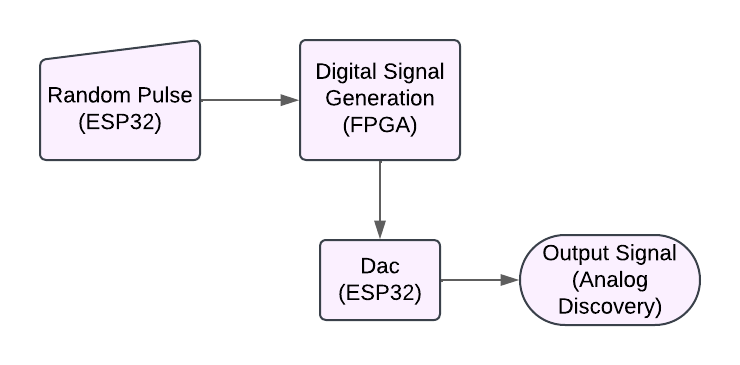
\includegraphics[scale=0.2]{diagrama_montaje_pulso.png}}
        \caption{Flujo de diseño para la generación de señales digitales}
        \label{flujo_de_diseño}
        \end{figure}



    \vspace{0.3cm}
   \subsection{Generación y procesamiento de señales}
    
    Mediante el ESP32 se producen pulsos aleatorios simulando eventos de detección de neutrinos y desencadenando el envio de señales digitales implementadas dentro del diseño de hardware mediante protocolo de comunicación UART hacia el ESP32.
        
    Se modela en lenguaje de descripción de hardware (HDL) una señal característica (Fig.~\ref{modeled_neutrino}) correspondiente a la respuesta de un SiPM (Silicon Photomultiplier) frente a la radiación de centelleo generada por la interacción de neutrinos con átomos de argón líquido. Los SiPM son fotodetectores de alta sensibilidad que consisten en una matriz de diodos de avalancha interconectados, capaces de amplificar la corriente producida por la detección de fotones.

    La corriente generada por los SiPM pasa a través de una etapa de amplificación de transimpedancia antes de ingresar a un AFE (Analog Front-End). A partir de la función de transferencia correspondiente (Eq.~\ref{eq_z_neutrino}), se obtiene la señal modelada, característica de este tipo de sistemas de adquisición. Dicha señal alcanza una amplitud máxima proporcional a la cantidad de electrones generados en respuesta a la radiación detectada y presenta una caída exponencial que da lugar a la descarga y recuperación del estado inicial del sistema.

            \subsubsection{Datos Predefinidos} Se desarrolla una entidad en VHDL que transmite un flujo continuo de datos previamente generados mediante simulaciones que implementan técnicas de Montecarlo usando el software de simulación para detectores basados en Argón liquido LArSoft y herramientas de análisis como MATLAB \cite{SiPMmatlab}, el cuál considera las condiciones de operación del detector, la sección eficaz y la energía resultante de las particulas en la interacción \cite{LArSoft}. Esta señal simulada consta de un arreglo de 630 datos, con un valor máximo de 255, adaptado para el DAC de 8 bits del ESP32. Este conjunto de datos se denomina  \textit{datos RAW}.
            
            \subsubsection{Datos por Ecuación en Diferencias} Estas entidades en VHDL generan señales basadas en un modelo descrito mediante ecuaciones en diferencias. Inicialmente, se implementa una señal de decaimiento exponencial, representada por la Eq.~\ref{eq:exp}, junto con su correspondiente ecuación en diferencias (Eq.~\ref{eq:exp_dif}).
            
            A partir de los datos simulados con LArSoft, se modela la señal de detección de las interacciones utilizando una ecuación en tiempo continuo que representa de forma simplificada pero aproximada la respuesta típica de los SiPM como se muestra en la Fig.~\ref{modeled_neutrino} y la ecuación Eq.~\ref{eq_neutrino_time}. Posteriormente, se aplica un proceso de discretización mediante la transformada Z, generando el modelo que permita adaptarse para ecuaciones en diferencias que a su vez pueda ser implementada en el sistema embebido. En particular esta ecuación de diferencias corresponde a la función de transferencia de la señal preamplificada que ingresa al AFE. Este enfoque y representación de señales es comunmente usado en el diseño de filtros digitales, además el respectivo diseño de la señal de detección se desglosa como se muestra en el diagrama de la Fig.~\ref{eq_dif_schematic}.
        
    \subsection {Transmisión mediante protocolo UART y conversión Digital-Analoga}
        
        Se implementa una entidad en VHDL que se encarga exclusivamente de gestionar una máquina de estados finita (FSM) de dos estados para que los datos entrantes se serializen en cadenas de bytes que sean transmitidas a través de un pin GPIO hacia la tarjeta que incorpora el ESP32 al baudrate máximo establecido por la configuración estándar del receptor (1Mbits/s). El baudrate de comunicacion se obtiene a partir de un divisor de reloj basado en el reloj principal de funcionamiento del sistema. El estado llamado dentro del VHDL $S0_{init}$ recibe los datos entrantes, los concatena con 2 bits conocidos como de bits de parada y siempre y cuando este habilitada la comunicación serial por medio de un puerto entrante, la FSM transita al estado $S1_{Datos}$ que envia por cada flanco del reloj saliente del divisor cada bit que compone la cadena finalizando en los 2 bits de parada y despues retorna al estado inicial para reiniciar el proceso de envio con otra muestra.
        
        Los datos recibidos mediante UART se envian del buffer de recepción al DAC integrado en el microprocesador, el cuál tiene una resolución de 8 bits, generando señales analógicas en el rango de 0V a 3.3V (normalizado a 1V), monitoreando la salida análoga a través del Analog Discovery 2.        

    



%En esta etapa del desarrollo, se realizaron pruebas iniciales enfocadas en la frecuencia de operación para cada componente del sistema, específicamente en los DACs, asegurando que fueran alimentados con las frecuencias correctas. Estos avances reflejan resultados positivos en el manejo de las señales de frecuencia, destacando la capacidad de los sistemas para operar de manera estable y precisa.

%Además, se están desarrollando sistemas complementarios para caracterizar los experimentos, alineados con las metodologías empleadas por otros integrantes del equipo de trabajo, quienes se enfocan en el análisis de señales específicas. 

% texto en ingles
%%%%%%%%%%%%%%%%%%%%%%%%%%%%%%%%%%%%%%%%%%%
%% Texto en ingles
%%%%%%%%%%%%%%%%%%%%%%%%%%%%%%%%%%%%%%%%%%%


This document presents an experimental validation of the test bench subsystem designed for the \textit{DAPHNE} boards that will be used in the DUNE experiment, specifically in the signal digitization phase. The methodology includes the procedures required to test simulated signals from neutrino events generated on FPGA-based hardware platforms. These signals are then converted to analog using an external DAC. The main steps of the experimental work are outlined below. % Este documento aborda una validación experimental del subsistema del banco de pruebas diseñado para las tarjetas DAPHNE que se utilizarán en el experimento DUNE, en particular en la fase de digitización de señales. La metodología incluye los procedimientos requeridos para probar señales simuladas de eventos de neutrinos generadas en plataformas de hardware basadas en FPGA. Posteriormente, estas señales se convierten en analógicas mediante un DAC externo. A continuación, se presentan los pasos principales del trabajo experimental.


    \subsection{Configuración del entorno experimental}
    
    El sistema experimental para las pruebas de generación de señales digitales, incluyen los siguientes componentes clave:
    \begin{itemize}
        \item Microcontrolador ESP32: Utilizado principalmente para aprovechar su DAC incorporado para procesar señales digitales generadas en un sistema externo al microprocesador. Este es programado con un FreeRTOS dedicado a las funciones de generación de eventos, tareas de adquisición y procesamiento mediante la plataforma de programación ESP-IDF (Espressif IoT Development Framework).
        
        \item Tarjeta de Desarrollo FPGA ARTY Z7 SoC Xilinx: Desde esta plataforma de hardware se realiza el diseño e implementación del sistema de generación de las señales digitales a procesar posteriormente.
        \item Analog Discovery 2: Instrumento utilizado para capturar la salida análogica generada mediante el DAC del microprocesador ESP32 y evaluar la fidelidad de la señal obtenida.
    \end{itemize}
    
    A continuación se observa un flujo de diseño de lo mencionado anteriormente.

    \vspace{0.3cm}

        \begin{figure}[H]
        \centerline{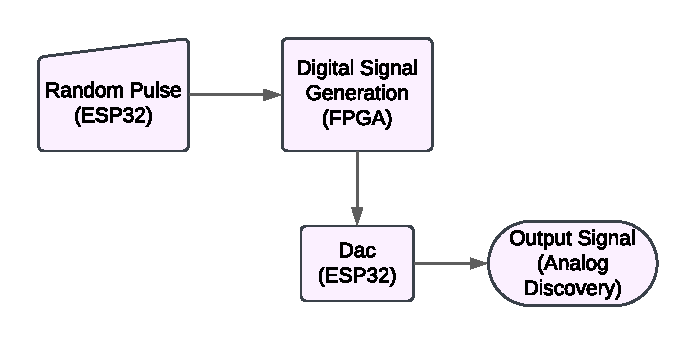
\includegraphics[scale=0.6]{montaje.pdf}}
        \caption{Flujo de diseño para la generación de señales digitales}
        \label{flujo_de_diseño}
        \end{figure}



    \vspace{0.3cm}
   \subsection{Generación y procesamiento de señales}
    
    Mediante el ESP32 se producen pulsos aleatorios simulando eventos de detección de neutrinos y desencadenando el envio de señales digitales implementadas dentro del diseño de hardware mediante protocolo de comunicación UART hacia el ESP32.
        
    Se modela en lenguaje de descripción de hardware (HDL) una señal característica (Fig.~\ref{modeled_neutrino}) correspondiente a la respuesta de un SiPM (Silicon Photomultiplier) frente a la radiación de centelleo generada por la interacción de neutrinos con átomos de argón líquido. Los SiPM son fotodetectores de alta sensibilidad que consisten en una matriz de diodos de avalancha interconectados, capaces de amplificar la corriente producida por la detección de fotones.

    La corriente generada por los SiPM pasa a través de una etapa de amplificación de transimpedancia antes de ingresar a un AFE (Analog Front-End). A partir de la función de transferencia correspondiente (Eq.~\ref{eq_z_neutrino}), se obtiene la señal modelada, característica de este tipo de sistemas de adquisición. Dicha señal alcanza una amplitud máxima proporcional a la cantidad de electrones generados en respuesta a la radiación detectada y presenta una caída exponencial que da lugar a la descarga y recuperación del estado inicial del sistema.

            \subsubsection{Datos Predefinidos} Se desarrolla una entidad en VHDL que transmite un flujo continuo de datos previamente generados mediante simulaciones que implementan técnicas de Montecarlo usando el software de simulación para detectores basados en Argón liquido LArSoft y herramientas de análisis como MATLAB \cite{SiPMmatlab}, el cuál considera las condiciones de operación del detector, la sección eficaz y la energía resultante de las particulas en la interacción \cite{LArSoft}. Esta señal simulada consta de un arreglo de 630 datos, con un valor máximo de 255, adaptado para el DAC de 8 bits del ESP32. Este conjunto de datos se denomina  \textit{datos RAW}.
            
            \subsubsection{Datos por Ecuación en Diferencias} Estas entidades en VHDL generan señales basadas en un modelo descrito mediante ecuaciones en diferencias. Inicialmente, se implementa una señal de decaimiento exponencial, representada por la Eq.~\ref{eq:exp}, junto con su correspondiente ecuación en diferencias (Eq.~\ref{eq:exp_dif}).
            
            A partir de los datos simulados con LArSoft, se modela la señal de detección de las interacciones utilizando una ecuación en tiempo continuo que representa de forma simplificada pero aproximada la respuesta típica de los SiPM como se muestra en la Fig.~\ref{modeled_neutrino} y la ecuación Eq.~\ref{eq_neutrino_time}. Posteriormente, se aplica un proceso de discretización mediante la transformada Z, generando el modelo que permita adaptarse para ecuaciones en diferencias que a su vez pueda ser implementada en el sistema embebido. En particular esta ecuación de diferencias corresponde a la función de transferencia de la señal preamplificada que ingresa al AFE. Este enfoque y representación de señales es comunmente usado en el diseño de filtros digitales, además el respectivo diseño de la señal de detección se desglosa como se muestra en el diagrama de la Fig.~\ref{eq_dif_schematic}.
        
    \subsection {Transmisión mediante protocolo UART y conversión Digital-Analoga}
        
        Se implementa una entidad en VHDL que se encarga exclusivamente de gestionar una máquina de estados finita (FSM) de dos estados para que los datos entrantes se serializen en cadenas de bytes que sean transmitidas a través de un pin GPIO hacia la tarjeta que incorpora el ESP32 al baudrate máximo establecido por la configuración estándar del receptor (1Mbits/s). El baudrate de comunicacion se obtiene a partir de un divisor de reloj basado en el reloj principal de funcionamiento del sistema. El estado llamado dentro del VHDL $S0_{init}$ recibe los datos entrantes, los concatena con 2 bits conocidos como de bits de parada y siempre y cuando este habilitada la comunicación serial por medio de un puerto entrante, la FSM transita al estado $S1_{Datos}$ que envia por cada flanco del reloj saliente del divisor cada bit que compone la cadena finalizando en los 2 bits de parada y despues retorna al estado inicial para reiniciar el proceso de envio con otra muestra.
        
        Los datos recibidos mediante UART se envian del buffer de recepción al DAC integrado en el microprocesador, el cuál tiene una resolución de 8 bits, generando señales analógicas en el rango de 0V a 3.3V (normalizado a 1V), monitoreando la salida análoga a través del Analog Discovery 2.        

    



%En esta etapa del desarrollo, se realizaron pruebas iniciales enfocadas en la frecuencia de operación para cada componente del sistema, específicamente en los DACs, asegurando que fueran alimentados con las frecuencias correctas. Estos avances reflejan resultados positivos en el manejo de las señales de frecuencia, destacando la capacidad de los sistemas para operar de manera estable y precisa.

%Además, se están desarrollando sistemas complementarios para caracterizar los experimentos, alineados con las metodologías empleadas por otros integrantes del equipo de trabajo, quienes se enfocan en el análisis de señales específicas. 








\section{Fundamentación Teórica }
\subsection{Transformada Z y Ecuacion en Diferencias}
La Transformada Z es una herramienta matemática esencial en el análisis de sistemas de tiempo discreto. Convierte una secuencia temporal \( x[n] \) en una representación algebraica en el dominio complejo \( z \), facilitando la resolución de ecuaciones en diferencias y el análisis dinámico de sistemas. Se define como:
\begin{equation}
    X(z) = \sum_{n=-\infty}^\infty x[n] z^{-n},
\end{equation}
donde \( z \) es una variable compleja. La Región de Convergencia (ROC) define el rango de valores de \( z \) donde la serie converge.

Una ecuación en diferencias describe la relación entre las muestras de entrada \( x[n] \) y salida \( y[n] \) en un sistema discreto. Por ejemplo, la ecuación:
\begin{equation}
    y[n] = x[n] + \sigma \cdot y[n-1],
\end{equation}
representa un sistema con retroalimentación, donde:
\begin{itemize}
    \item \( x[n] \) es la entrada actual,
    \item \( \sigma \) es un parámetro que determina la influencia de la salida pasada \( y[n-1] \),
    \item \( y[n] \) es la salida actual.
\end{itemize}

La Transformada Z permite analizar esta relación en el dominio \( z \). Aplicando la Transformada Z a ambos lados de la ecuación y usando las propiedades de desplazamiento temporal:
\begin{equation}
    \mathcal{Z}\{y[n]\} = \mathcal{Z}\{x[n]\} + \sigma \mathcal{Z}\{y[n-1]\}.
\end{equation}
Sustituyendo las propiedades de la Transformada Z:

\begin{equation}
    Y(z) = X(z) + \sigma z^{-1} Y(z).
\end{equation}
Esta ecuación en el dominio \( z \) describe cómo la salida \( Y(z) \) depende de la entrada \( X(z) \) y de la retroalimentación en \( \sigma z^{-1} Y(z) \) \cite{proakis2007tratamiento}.
\subsection{Evaluación de eficiencia, consumo de área y recursos de hardware de las entidades HDL}
Se tiene como objetivo mostrar las métricas de consumo de recursos y cumplimiento de tiempos en el transporte de señales con cada una de las entidades VHDL implementadas en la FPGA generando una comparación entre las 2 opciones previamente establecidas:

\begin{itemize}
    \item \textbf{Look-Up Tables (LUTs):} 
    Son bloques de hardware de la lógica programable que implementan funciones combinacionales. Su uso ideal no debe superar el 70\% de la capacidad total para evitar problemas de enrutamiento y asegurar la eficiencia del diseño.  
    
    \item \textbf{Flip-Flops (FFs):} 
    Los FFs son elementos de almacenamiento secuencial que retienen un bit de información y forman los registros del sistema. Trabajan con las LUTs para implementar la lógica secuencial. Es importante equilibrar su uso con el de las LUTs para evitar problemas en la arquitectura o asignación de recursos.

    \item \textbf{LUTRAM:} 
    Es una funcionalidad que permite utilizar las LUTs como bloques de memoria RAM. Esto es útil para el almacenamiento temporal de datos, aprovechando los recursos existentes sin requerir memoria adicional. Sin embargo, su uso excesivo puede limitar la lógica disponible para otras funciones.

    \item \textbf{DSP (Digital Signal Processing):} 
    Son bloques especializados para realizar operaciones matemáticas complejas como multiplicaciones y sumas acumulativas. Su uso es clave en aplicaciones que requieren alto desempeño en cálculos, como procesado de señales o algoritmos científicos.

    \item \textbf{Worst Negative Slack (WNS):} 
    Representa el mayor incumplimiento de tiempo en las rutas críticas que conforman el diseño. Un valor mayor o igual a 0 indica que todas las rutas cumplen con los tiempos establecidos, garantizando que el diseño funcione correctamente a la frecuencia de base deseada.

    \item \textbf{Total Negative Slack (TNS):} 
    Es la suma de todos los incumplimientos de tiempo en el diseño. Un valor de 0 significa que no existen violaciones de tiempo en ninguna de las rutas.\cite{xilinx_clb_guide}
\end{itemize}

  




\section{Resultados}

        \begin{figure}[H]
        \centerline{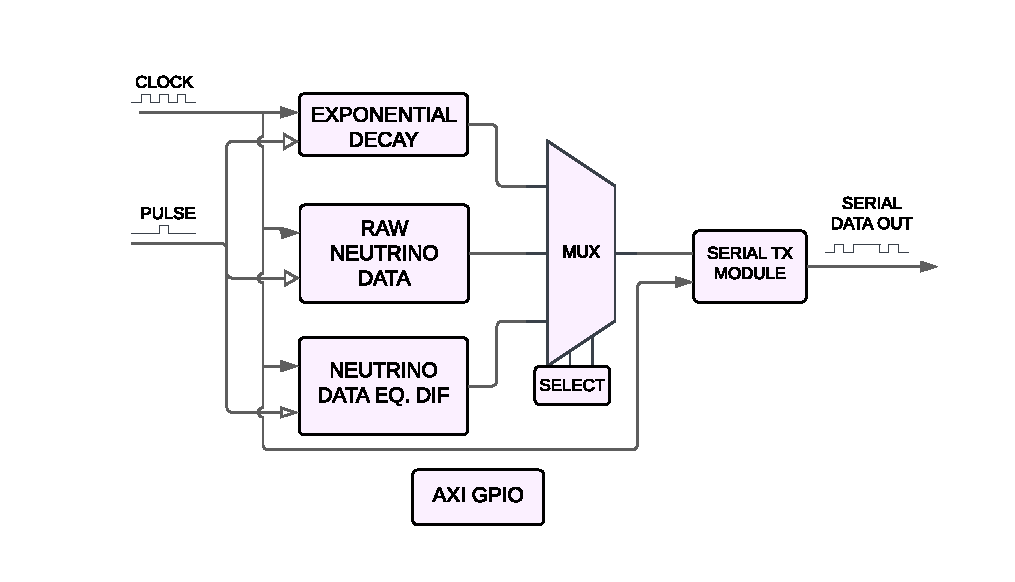
\includegraphics[scale=0.55]{Diagrama_vivado.pdf}}
        \caption{Esquematico del diseño final construido en Vivado 2022.1}
        \label{vivado_sch}
        \end{figure}

Se implementa y se configura el sistema embebido mediante el Software Vivado 2022.2 con el diseño de hardware que se muestra en la Fig.~\ref{vivado_sch} el cuál integra el conjunto de bloques generadores de las señales \textit{EXPONENTIAL DECAY, RAW NEUTRINO DATA, NEUTRINO DATA EQ. DIF.} mediante los métodos descritos y se seleccionan para salida de datos con un multiplexor 4 a 1 conectado al bloque de diseño y controlado mediante un AXI GPIO que permite establecer la selección por medio del sistema operativo el cual es un entorno de jupyter. \textit{SERIAL TX MODULE} mediante protocolo UART recibe el dato y lo serializa en cadena de bits enviandolo a través del pin GPIO hacia el ESP32. Las entidades de hardware se sincronizan mediante señales de control como un reloj principal \textit{CLOCK} y la que establece la condición de reseteo en cada entidad, \textit{RESET}.

\textit{PULSE} indica el pulso proveniente del ESP32 que dispara la generación de la señal seleccionada. El FreeRTOS implementado en el ESP32 dedica una tarea especifica a generar el pulso de activación de forma intermitente en intervalos de tiempo aleatorios mediante el uso de un TRNG (True Random Number Generator) incorporado dentro de la tarjeta de desarrollo del microprocesador. 

\subsection{Fase 1: Exponencial Decreciente por Ecuación en Diferencias}
Inicialmente se hace la implementación del sistema de generación y transmisión con el diseño de hardware correspondiente a la exponencial decreciente que se presenta en la Eq.~\ref{eq:exp}. La ecuación en diferencias asociada a esta señal aplicando la transformación Z se expresa como se sigue en la Eq.~\ref{eq:exp_dif} que incluye retroalimentación con base al resultado anterior n-1 y un factor de decaimiento \( \sigma \) = 0.99.

\begin{equation}
    f(x) = e^{-0.99x}
    \label{eq:exp}
\end{equation}

\begin{equation}
    y[n] = x[n] + 0.99 \cdot y[n-1]
    \label{eq:exp_dif}
\end{equation}

Para implementar el modelo segun la Eq.~\ref{eq:exp_dif} en VHDL se utiliza una máquina de estados finitos (FSM) que gestiona la evolución de los cálculos, comenzando desde un valor inicial predefinido establecido por $y[0]$ y recalculando el valor $y[n]$ de forma iterativa por cada ciclo de reloj, finalmente el vector de bits resultante se trunca en 8 bits asignandose a la salida que conecta con el módulo de comunicación serial. La arquitectura del módulo se comopone de una FSM de cuatro estados: \( S_{rst}, S0, S1, \) y \( S2 \).

\begin{itemize}
    \item \textbf{Estado \( S_{rst} \):} Se restablecen las variables del sistema a sus valores iniciales, regresando así el módulo a un estado inicial.
    \item \textbf{Estado \( S0 \):} La salida se inicializa en el valor pico cuando se detecta un nuevo pulso en la entrada de trigger y se transita al estado \( S1 \)
    \item \textbf{Estado \( S1 \):} Se realiza la recurrencia de la ecuación en diferencias, actualizando la salida hasta que el valor calculado llegue a cero.
    \item \textbf{Estado \( S2 \):} La salida se pone en cero, permaneciendo en este estado indefinidamente hasta que se detecte un nuevo pulso o se indique el regreso del sistema al estado inicial.
\end{itemize}


\begin{figure}[H]
\centerline{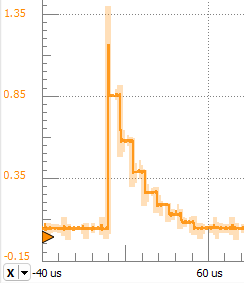
\includegraphics[scale=0.5]{exponencial_signal.png}}
        \caption{Señal Exponencial Decreciente en Analog Discovery 2}
        \label{exponencial_signal}
        \end{figure}


\subsection{Fase 2: Señal de detección de Neutrinos}


\subsubsection{Generación de Datos}
Posterior a la implementación de la señal exponencial, se procede a utilizar los datos generados mediante LArSoft de la señal simulada para crear la entidad en VHDL que realize el stream de los mismos hacia la etapa del DAC. Los 630 datos se establecen en un array interno que como componente de hardware se puede ver como un banco de registros que almacena los datos y se accede mediante una estructura multiplexora. Al activarse el pulso de detección desde el ESP32, se envia al puerto de salida el vector de 8 bits equivalente al dato tipo integer dentro del array y por medio de un indice que recorre las pocisiones de este arreglo se envian continuamente los datos actualizando la salida por cada ciclo del reloj que gobierna la ejecución del diseño de hardware. Al terminar el stream de datos del array, se establece la salida de datos en cero hasta la detección de un nuevo evento y reiniciar el stream \hl{citar repositorio GitHub}


\subsubsection{Modelo matemático de ajuste a la señal}
Con los datos generados en LArSoft se modela la señal de detección en tiempo continuo como se muestra en la Eq.~\ref{eq_neutrino_time}.

\begin{figure}[htpb]
    \centerline{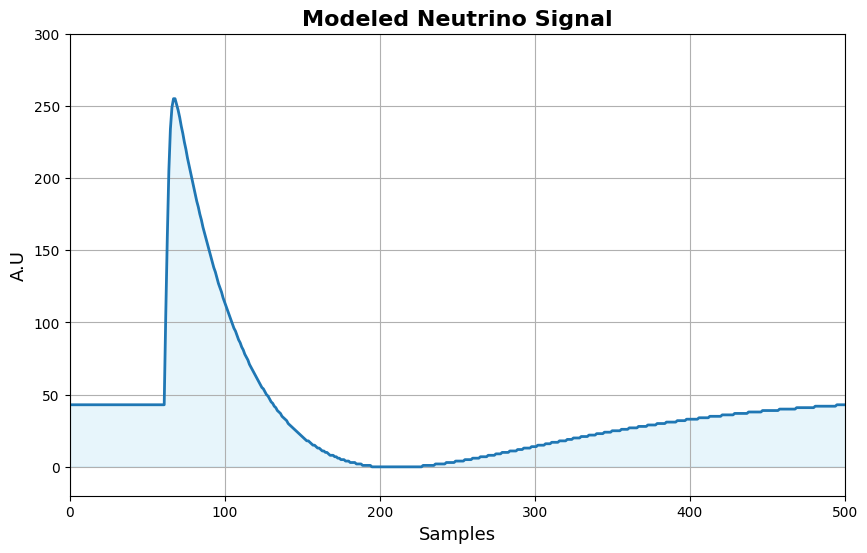
\includegraphics[scale=0.35]{modeled_neutrino_signal.png}}
    \caption{Señal de respuesta SiPM ante un evento de detección.}
    \label{modeled_neutrino}
\end{figure}


\begin{equation}
\label{eq_neutrino_time}
y(t) = (C_2  e^{-a_2 (t - d)} \cos(a_2  (t - d)) - C_1 e^{-a_1 (t - d)})\cdot u(t-d)
\end{equation}

Donde $C_1$ y $C_2$ respresentan la amplitud efectiva de una señal biexponencial mostrada en la Fig.~\ref{modeled_neutrino}, $a_1$ representa la constante de tiempo de ascenso de la señal, $a_2$ la constante de tiempo de descenso de la señal exponencial, $d$ representa el tiempo de ocurrencia del evento y $u(t-d)$ es la funcion de Heaviside retrasada. Se llevo a cabo un proceso de ajuste por minimos cuadrados para encontrar los valores mas adecuados para cada una de las constantes involucradas en el modelo. En la Tabla \ref{tab_biexp} se presenta el valor para estas constantes.




\begin{table}[htbp]
\caption{Valor estimado para las constantes involucradas en el modelo matematico de la respuesta de los SiPM frente a la interaccion de Neutrinos}
\begin{center}
\begin{tabular}{|c|c|c|c|c|}
\hline
$C_1$ & $C_2$ & $a_1$ & $a_2$ & $d$ \\
\hline
$41.83$ & $40.45$ & $31.84$ & $7.86$ & $0.11$ \\
\hline
\end{tabular}
\label{tab_biexp}
\end{center}
\end{table}

Posteriormente se realiza la discretización de la señal mediante la aplicación de la transformada Z, obteniendo así el modelo de ecuación en diferencias adaptado para implementarse en VHDL, el cuál se muestra en la ecuación \ref{eq_z_neutrino}

\begin{equation}
\small
\label{eq_z_neutrino}
\frac{Y(z)}{X(z)}= \dfrac{K_1 + K_2 z^{-1} + K_3 z^{-2} +K_4 z^{-3} +K_5 z^{-4}}{C_1 + C_2 z^{-1} + C_3 z^{-2} +C_4 z^{-3} +C_5 z^{-4}}
\end{equation}

{Donde $C_1$, $C_2$, $C_3$, $C_4$, $C_5$ corresponden a los coeficientes de ponderación de los datos de respuesta anteriores producidos por el modelo, $K_1$, $K_2$, $K_3$, $K_4$, $K_5$ representan los coeficientes de ponderacion de los datos de la señal de entrada, que para el caso de este modelo corresponde a un impulso unitario $\delta(t-d)$. En la tabla \ref{tab_coef_z_neutrino} se preserntan los valores para los coeficientes del modelo discreto de la señal de detección de neutrinos.

\begin{table}[htbp]
\caption{Valor estimado para las constantes involucradas en el modelo matematico discretizado de la respuesta de los SiPM frente a la interaccion de Neutrinos}
\begin{center}
\begin{tabular}{|c|c|c|c|c|}
\hline
$C_1$ & $C_2$ & $C_3$ & $C_4$ & $C_5$ \\
\hline
$33554432$ & $-85042484$ & $54221008$ & $12468155$ & $15201111$ \\
\hline
\hline
$K_1$ & $K_2$ & $K_3$ & $K_4$ & $K_5$ \\
\hline

$33554432$ & $-131839891$ & $194240369$ & $-127178346$ & $31223436$ \\
\hline
\end{tabular}
\label{tab_coef_z_neutrino}
\end{center}
\end{table}

\subsection{Fase 3: Implementación en HDL de la Ecuación en Diferencias para Detección de Neutrinos}
 \begin{figure}[H]
\centerline{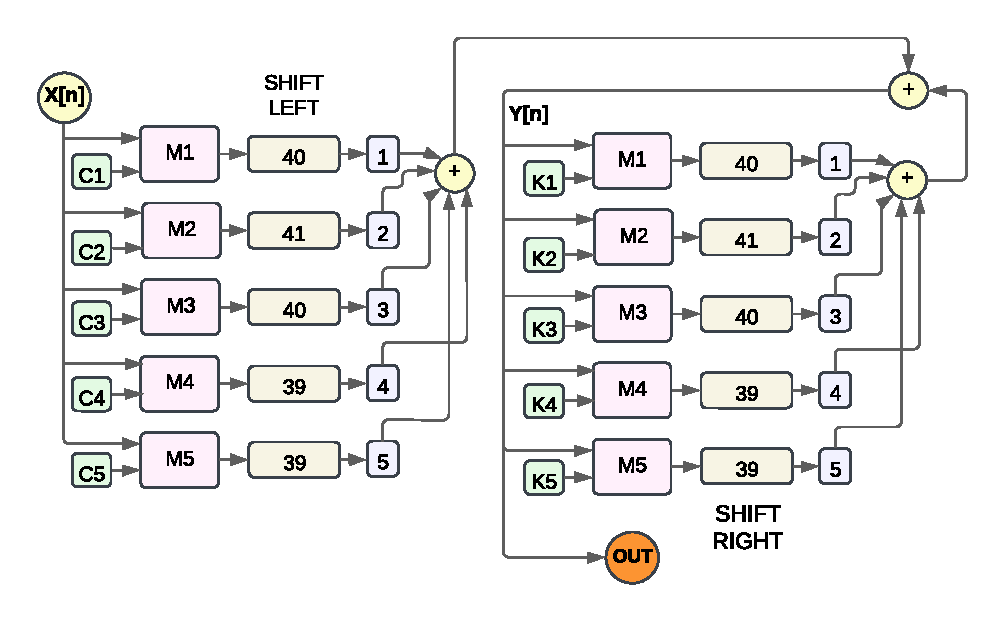
\includegraphics[scale=0.5]{eq_dif_vhdl_diagram.pdf}}
        \caption{Diagrama Diseño HDL de ecuación en diferencias señal de detección}
        \label{eq_dif_schematic}
        \end{figure}
        
De acuerdo a la Fig.~\ref{eq_dif_schematic} la implementación en hardware del filtro dada ecuación en diferencias en la Eq.~\ref{eq_z_neutrino} se hace por medio de una estructura que tiene una serie de entidades multiplicadoras M1, M2, M3, M4, M5 que operan la señal respuesta anterior X[n] con cada constante $C_{i}$, cada una de las salidas de estas operaciones se retardan por desplazamiento de registros correspondiente a las muestras generadas en el tiempo discreto X[n-1], X[n-2], ..., X[n-i] y los valores númericos en las etapas de retardo como se muestran en la Fig.~\ref{eq_dif_schematic} corresponden con la longitud en bits que manejan los registros en cada una de las etapas. Las salidas de las etapas anteriores pasan a un sumador que envia el resultante a otro sumador que opera esta señal con la salida correspondiente de las etapas de multiplicación, retardo por desplazamiento y suma de los datos de la señal de entrada Y[n], de donde la señal resultante es la respuesta final que se envia para retroalimentar de nuevo las etapas mencionadas y actualizar la salida, además la señal que sale del último sumador se trunca a 8 bits para asignarse al puerto de salida que se interconecta con el módulo de comunicación UART y obtener asi el dato a enviar mediante serialización. \hl{REVISAR COMPLEMENTAR FABIAN}

Finalmente mediante monitoreo constante con el Analog Discovery 2 se obtienen las señales analogas salientes del DAC las que se muestran en las Fig.~\ref{predefined_neutrino} y Fig.~\ref{eq_dif_neutrino_img}.

\begin{figure}[H]
\centerline{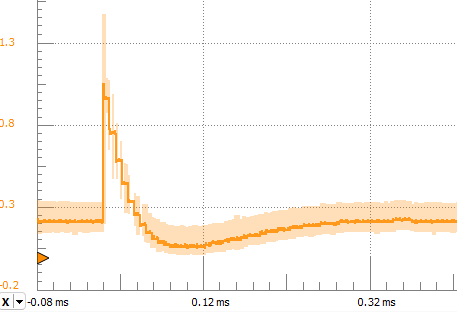
\includegraphics[scale=0.5]{datos_predefinidos_analog.png}}
        \caption{Salida análoga - señal generada con datos RAW}
        \label{predefined_neutrino}
        \end{figure}

\begin{figure}[H]
\centerline{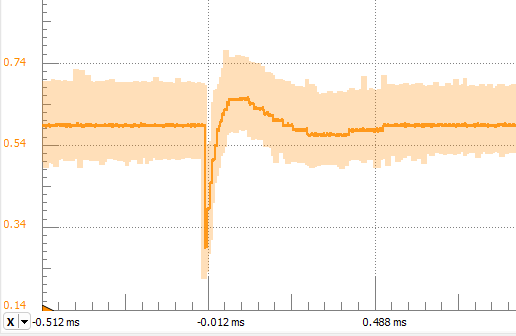
\includegraphics[scale=0.4]{signal_eq_dif.png}}
        \caption{Salida análoga - señal generada mediante ecuación en diferencias.}
        \label{eq_dif_neutrino_img}
        \end{figure}

Dadas las señales respuesta análogicas se determina un rango aproximado para la frecuencia de conversión del DAC incorporado dentro del ESP32. Haciendo la medida del tiempo que dura cada muestra para cada señal se obtienen intervalos que oscilan entre $6.8\mu s$ y $7.0\mu s$ lo cual permite determinar un rango de frecuencias de conversión entre 140kHz y 147kHz, lo cuál en comparación con la máxima frecuencia de muestreo del Analog Discovery que es de 100MHz garantiza una adquisición confiable de los datos de la señal sin efectos de aliasing.

Posterior a testear cada unos de los diseños de hardware para la generación de las señales, se integra el diseño final que corresponde al mostrado en la Fig.~\ref{vivado_sch} el cuál funciona correctamente de acuerdo a los esperado.

\subsection{Fase 4: Evaluación de la eficiencia de los diseño de hardware para la generación de señales}
\subsubsection{Diseño HDL con Datos Predefinidos}
para la entidad denominada \textit{RAW Neutrino data} se obtienen los parámetros descritos en la Tabla~\ref{predefined data evaluation} los cuales se obtienen haciendo el proceso de Implementación en Vivado 2022.2 lo que incluye uso de recursos de Hardware (LUTs, FFs, RAM...) y la evaluación del cumplimiento de tiempos en las rutas generadas para el transporte de las señales (WNS, TNS).




\begin{table}[H]
\caption{Uso de Recursos de FPGA para señal generada con datos RAW}
\begin{center}
\begin{tabular}{|c|c|c|c|}
\hline
\textbf{Resource} & \textbf{Utilization} & \textbf{Avaliable} & \textbf{\% Utilization} \\
\hline
\textbf{LUT} & 70 & 53200 & 0.13 \\
\hline
\textbf{FF} & 50 & 106400 & 0.05 \\
\hline
\end{tabular}
\label{predefined data evaluation}
\end{center}
\end{table}

\begin{itemize}
  \item \textbf{Worst Negative Slack (WNS):}
    \begin{itemize}
        \item Para el \textit{Setup Timing}, el valor tiende a infinito, lo que significa que no hay rutas críticas con incumplimientos de tiempo negativo, y el diseño cumple con los tiempos de configuración.
        \item Para el \textit{Hold Timing}, el valor también es infinito, indicando que no hay violaciones de retención en las rutas y cumpliendo con las condiciones de retardo mínimo en el transporte de las señales.
    \end{itemize}
    
    \item \textbf{Total Negative Slack (TNS):}
    \begin{itemize}
        \item Para el \textit{Setup Timing}, el valor es 0 ns, lo que indica que no hay acumulación de retrasos en ninguna de las rutas.
        \item Para el \textit{Hold Timing}, también es 0 ns, lo que significa que no hay acumulación de violaciones de retención en las señales.
    \end{itemize}
\end{itemize}

\subsubsection{Diseño HDL por ecuación en diferencias de la señal}

\begin{table}[H]
\caption{Uso de Recursos de FPGA para señal generada por ecuación en diferencias}
\begin{center}
\begin{tabular}{|c|c|c|c|}
\hline
\textbf{Resource} & \textbf{Utilization} & \textbf{Avaliable} & \textbf{\% Utilization} \\
\hline
\textbf{LUT} & 473 & 53200 & 0.89 \\
\hline
\textbf{LUTRAM} & 156 & 17400 & 0.90 \\
\hline
\textbf{FF} & 793 & 106400 & 0.75 \\
\hline
\textbf{DSP} & 25 & 220 & 11.36 \\
\hline
\end{tabular}
\label{eq_dif_table_evaluation}
\end{center}
\end{table}

 




\begin{itemize}
  \item \textbf{Worst Negative Slack (WNS):}
    \begin{itemize}
        \item Para el \textit{Setup Timing}, el valor es $2.283 \, \text{ns}$, lo que indica que existe una pequeña ruta crítica con incumplimiento temporal, pero dentro de límites manejables para la mayoría de aplicaciones.
        \item Para el \textit{Hold Timing}, el valor es $0.030 \, \text{ns}$, mostrando una ligera violación de retención que puede requerir ajustes en el diseño.
    \end{itemize}
    
    \item \textbf{Total Negative Slack (TNS):}
    \begin{itemize}
        \item Para el \textit{Setup Timing}, el valor es 0 ns, lo que indica que no hay acumulación de retrasos significativos en las rutas.
        \item Para el \textit{Hold Timing}, también es 0 ns, lo que significa que no hay acumulación de violaciones de retención.
    \end{itemize}
\end{itemize}






\section{Discusión}

\subsection{Generación de señales implementadas en HDL}

Se confirma la correcta implementación de la ecuación en diferencias basada en la transformación Z, lo cuál es evidenciado durante la simulación e implementación del hardware para la señal de decaimiento exponencial, además de corroborarse con la medición analogica de la señal resultante que puede verse en la Fig.~\ref{exponencial_signal}. En cuanto a lo que tiene que ver con la resolución de los datos generados esta se encuentra limitada al rango de representación entera no signada en 8 bits que corresponde a valores desde 0 a 255. 

La Fig.~\ref{predefined_neutrino} muestra claramente la señal respuesta de los SiPM ante un evento de detección, posterior a la etapa de conversión Digital-Análoga en el DAC de la ESP32. La señal obtenida es una evidencia clara del funcionamiento esperado del diseño de hardware que hace el stream de los datos RAW de la señal. Este comportamiento indica que la implementación práctica del modelo cumple con los objetivos planteados y que el hardware reproduce con precisión las características esperadas.

El análisis de la señal confirma que el sistema no presenta comportamientos irregulares excluyendo de ello las fuentes de ruido parásito presentes en la señal. Se demuestra además la correcta configuración y funcionamiento del DAC de la ESP32, así como la efectividad del modelo implementado para generar la salida observada.

La Fig.~\ref{eq_dif_neutrino_img} presenta los resultados obtenidos mediante la implementación del diseño de hardware de la ecuación en diferencias derivada de la transformación Z, procesada por el sistema embebido y convertida a señal analógica. El comportamiento observado valida la correcta implementación del modelo matemático en el sistema de hardware reconfigurable, ya que los datos muestran un comportamiento coherente con lo esperado al aplicar el proceso de filtrado. La respuesta del sistema modelado además de evidenciar la precisión en la discretización de los datos tambien presenta correcta estabilidad del diseño en funcionamiento. La salida de datos se encuentra truncada a 8 bits a partir de un valor con representación de 64 bits, lo que claramente refleja una disminución considerable en la resolución de la representación de la señal pero que no elimina las caracteristicas principales a preservar en la señal lo cual se observa claramente en la Fig.~\ref{eq_dif_neutrino_img}.

Se aclara que a pesar de que en este proyecto se estan implementando la generación de señales con datos de 8 bits, también se puede realizar mediante datos con representaciones de mayor orden y asi mejorar la resolución de las señales de salida, sin embargo esto contemplaria modificaciones en la lógica del diseño HDL que gestiona el envio de datos serializados (TX) asi como la configuración de los parámetros del ESP32 como receptor (RX) para concatenar palabras de mayor longitud, teniendo presente que esto se hace en la medida de las necesidades de velocidad o fidelidad de las señales generadas.

\subsection{Comparación de las Implementaciones de los diseños HDL}

El diseño implementado con datos RAW utiliza una cantidad mínima de recursos de la FPGA en comparación con la capacidad total disponible lo que se puede ver en la Tabla~\ref{predefined data evaluation}, lo que sugiere un diseño compacto en términos de uso de registros y otros recursos de hardware que componen la FPGA, además, no presenta violaciones de tiempo de acuerdo a los parámetros TNS y WNS arrojados durante el proceso de implementación, garantizando que todas las rutas de las señales estan cumpliendo con las condiciones de temporización y garantiza que el diseño es completamente funcional tanto en \textit{setup timing} (tiempos de configuración) como en \textit{hold timing} (tiempos de retención).

A diferencia del diseño HDL con los datos RAW, la implementación con el modelo de ecuación en diferencias (Fig.~\ref{eq_dif_schematic}) implica un uso considerablemente mayor de recursos debido al procesamiento dinámico de las ecuaciones en diferencias lo cual se puede reflejar en el uso de DSPs (Digital Signal Processing) en la Tabla~\ref{eq_dif_table_evaluation} que presenta un porcentaje de utilización de 11.36\% dado que se integran diferentes etapas de operaciones de las señales como multiplicadores y sumadores, también se destaca que debido a la representación de alto orden de las constantes dadas por la Tabla~\ref{tab_coef_z_neutrino} y el cuantioso uso de registros para almacenar las señales intermedias, el uso de LUTs, FFs aumenta además de también tenerse un uso de bloques de LUTRAM, lo que representa un consumo energetico mas alto en comparación con la implementación de datos RAW.

Los parámetros de temporización WNS, TNS en el diseño por ecuación en diferencias si presentan algunas rutas para transportar señales que no cumplen los requerimientos establecidos además de tambien tenerse violaciones en tiempos de retención y retardo debido a que esta implementación de hardware es mas robusta que la anterior, sin embargo al analizar el parámetro TNS se determina que no existen incumplimientos que generen acumulaciones de ineficiencias en tiempo para la totalidad del diseño y que en conjunto, este cumple con los parámetros de temporización.

El diseño basado en datos RAW destaca por su eficiencia en el uso de recursos y bajo consumo energético, siendo ideal para aplicaciones compactas con restricciones de hardware y energía. Por otro lado, el diseño basado en ecuaciones en diferencias ofrece una mayor capacidad de procesamiento dinámico en tiempo real, precisión en sistemas complejos y escalabilidad, lo que lo hace adecuado para aplicaciones más exigentes y versátiles en procesamiento de señales acotando que la paralelización de su ejecución en sistemas que integran FPGAS permite que estas implementaciones sean muy eficientes. La elección entre ambos depende del balance entre los recursos disponibles y los requerimientos funcionales del sistema.

% \section*{References}

% Please number citations consecutively within brackets \cite{b1}. The 
% sentence punctuation follows the bracket \cite{b2}. Refer simply to the reference 
% number, as in \cite{b3}---do not use ``Ref. \cite{b3}'' or ``reference \cite{b3}'' except at 
% the beginning of a sentence: ``Reference \cite{b3} was the first $\ldots$''

% Number footnotes separately in superscripts. Place the actual footnote at 
% the bottom of the column in which it was cited. Do not put footnotes in the 
% abstract or reference list. Use letters for table footnotes.

% Unless there are six authors or more give all authors' names; do not use 
% ``et al.''. Papers that have not been published, even if they have been 
% submitted for publication, should be cited as ``unpublished'' \cite{b4}. Papers 
% that have been accepted for publication should be cited as ``in press'' \cite{b5}. 
% Capitalize only the first word in a paper title, except for proper nouns and 
% element symbols.

% For papers published in translation journals, please give the English 
% citation first, followed by the original foreign-language citation \cite{b6}.



\bibliographystyle{IEEEtran}  % Estilo de citas IEEE
\bibliography{referencias}  % Nombre de tu archivo .bib (sin la extensión .bib)


% [1] https://arxiv.org/abs/2002.03010
% [2] S. Asai, et al., Exploring the quantum universe, ³Report of the 2023 Particle Physics Project
% Prioritization Panel´, 2023, Disponible: https://www.usparticlephysics.org/2023-p5-report/
% [3] A. Abed, et al., DUNE Collaboration, ³DUNE Phase II: Scientific Opportunities, Detector Concepts,
% Technological SRlXWiRnV ³, 2024, Disponible: http://arxiv.org/abs/2408.12725
% [4] https://arxiv.org/abs/1205.6747
% [5] https://www.st.com/en/microcontrollers-microprocessors/stm32h753ii.html#documentation
% [6]https://www.amd.com/es/products/adaptive-socs-and-fpgas/fpga/artix-7.html
% [7] B. Abi et al., ³Deep Underground Neutrino Experiment (DUNE), Far Detector TechnicalDesign
% Report, Volume IV: Far Detector Single-phase Technology.´ arXiv, 2020.
% [8] Li.Jiaying, et al., ³Research on Fault Prediction and Health Management of Power Supply Board Method Based on Mahalanobis Distance³ https://www-scopus-com.udea.lookproxy.com/record/display.uri?eid=2-s2.0-85205504247&origin=resultslist&sort=plf-f&src=s&sid=c31314c1e8950e998323826a91fe80ec&sot=a&sdt=cl&cluster=scosubtype%2C%22ar%22%2Ct%2C%22cp%22%2Ct%2Bscolang%2C%22English%22%2Ct%2Bscoexactkeywords%2C%22Fault+Detection%22%2Ct&s=TITLE-ABS-KEY+%28+%28+%22artificial+intelligence%22+OR+%22predict%22+OR+%22System%22+OR+%22Machine+Learning%22%29+AND+%28+%22electronic+boards%22+OR+%22PCBs%22+OR+%22circuit+boards%22+%29+%29+AND+PUBYEAR+%26gt%3B+1995+AND+PUBYEAR+%26lt%3B+2025&sl=195&sessionSearchId=c31314c1e8950e998323826a91fe80ec&relpos=3
% [10] G. Esteban Ferrer, ³Diseño e implementación de un circuito electrónico en FPGA para la
% optimización de la detección de eventos en el experimento de física de partículas NEXT (Neutrino
% Experiment with a Xenon TPC)´, p. 110279, 2018.





% \begin{thebibliography}{00}
% \bibitem{b1} G. Eason, B. Noble, and I. N. Sneddon, ``On certain integrals of Lipschitz-Hankel type involving products of Bessel functions,'' Phil. Trans. Roy. Soc. London, vol. A247, pp. 529--551, April 1955.
% \bibitem{b2} J. Clerk Maxwell, A Treatise on Electricity and Magnetism, 3rd ed., vol. 2. Oxford: Clarendon, 1892, pp.68--73.
% \bibitem{b3} I. S. Jacobs and C. P. Bean, ``Fine particles, thin films and exchange anisotropy,'' in Magnetism, vol. III, G. T. Rado and H. Suhl, Eds. New York: Academic, 1963, pp. 271--350.
% \bibitem{b4} K. Elissa, ``Title of paper if known,'' unpublished.
% \bibitem{b5} R. Nicole, ``Title of paper with only first word capitalized,'' J. Name Stand. Abbrev., in press.
% \bibitem{b6} Y. Yorozu, M. Hirano, K. Oka, and Y. Tagawa, ``Electron spectroscopy studies on magneto-optical media and plastic substrate interface,'' IEEE Transl. J. Magn. Japan, vol. 2, pp. 740--741, August 1987 [Digests 9th Annual Conf. Magnetics Japan, p. 301, 1982].
% \bibitem{b7} M. Young, The Technical Writer's Handbook. Mill Valley, CA: University Science, 1989.
% \end{thebibliography}
% \vspace{12pt}
% \color{red}
% IEEE conference templates contain guidance text for composing and formatting conference papers. Please ensure that all template text is removed from your conference paper prior to submission to the conference. Failure to remove the template text from your paper may result in your paper not being published.



\end{document}





















\documentclass[onecolumn]{IEEEtran}
\IEEEoverridecommandlockouts
% The preceding line is only needed to identify funding in the first footnote. If that is unneeded, please comment it out.
\usepackage{cite}
\usepackage{amsmath,amssymb,amsfonts}
\usepackage{algorithmic}
\usepackage{graphicx}
\usepackage{textcomp}
\usepackage{xcolor}
\def\BibTeX{{\rm B\kern-.05em{\sc i\kern-.025em b}\kern-.08em
    T\kern-.1667em\lower.7ex\hbox{E}\kern-.125emX}}

\title{\boldmath  \\
{\footnotesize \textsuperscript{} }}


\begin{document}

\maketitle

\section{Resumen}

\vspace{0.5cm}




\end{document}

